%%%%%%%%%%%%%%%%%%%%%%%%%%%%%%%%%%%%%%%%%%%%%%%%%%%%%%%%%%%%%%%%%%%%%%%%%%%%
%% Author template for INFORMS Journal on Computing (ijoc)
%% Mirko Janc, Ph.D., INFORMS, mirko.janc@informs.org
%% ver. 0.95, December 2010
%%%%%%%%%%%%%%%%%%%%%%%%%%%%%%%%%%%%%%%%%%%%%%%%%%%%%%%%%%%%%%%%%%%%%%%%%%%%
%\documentclass[ijoc,blindrev]{informs3}
\documentclass[ijoc,nonblindrev]{informs3} % current default for manuscript submission

%%\OneAndAHalfSpacedXI
\OneAndAHalfSpacedXII % current default line spacing
%%\DoubleSpacedXII
%%\DoubleSpacedXI

% If hyperref is used, dvi-to-ps driver of choice must be declared as
%   an additional option to the \documentclass. For example
%\documentclass[dvips,ijoc]{informs3}      % if dvips is used
%\documentclass[dvipsone,ijoc]{informs3}   % if dvipsone is used, etc.

% Private macros here (check that there is no clash with the style)
\usepackage[]{algorithm2e}
\usepackage{hyperref}
\graphicspath{images/}
\usepackage{caption}

% Natbib setup for author-year style
\usepackage{natbib}
 \bibpunct[, ]{(}{)}{,}{a}{}{,}%
 \def\bibfont{\small}%
 \def\bibsep{\smallskipamount}%
 \def\bibhang{24pt}%
 \def\newblock{\ }%
 \def\BIBand{and}%

%% Setup of theorem styles. Outcomment only one. 
%% Preferred default is the first option.
\TheoremsNumberedThrough     % Preferred (Theorem 1, Lemma 1, Theorem 2)
%\TheoremsNumberedByChapter  % (Theorem 1.1, Lema 1.1, Theorem 1.2)

%% Setup of the equation numbering system. Outcomment only one.
%% Preferred default is the first option.
\EquationsNumberedThrough    % Default: (1), (2), ...
%\EquationsNumberedBySection % (1.1), (1.2), ...

% In the reviewing and copyediting stage enter the manuscript number.
\MANUSCRIPTNO{42} % When the article is logged in and DOI assigned to it,
                 %   this manuscript number is no longer necessary

%%%%%%%%%%%%%%%%
\begin{document}
%%%%%%%%%%%%%%%%

% Outcomment only when entries are known. Otherwise leave as is and 
%   default values will be used.
%\setcounter{page}{1}
%\VOLUME{00}%
%\NO{0}%
%\MONTH{Xxxxx}% (month or a similar seasonal id)
\YEAR{2015}% e.g., 2005
%\FIRSTPAGE{000}%
%\LASTPAGE{000}%
%\SHORTYEAR{00}% shortened year (two-digit)
%\ISSUE{0000} %
%\LONGFIRSTPAGE{0001} %
%\DOI{10.1287/xxxx.0000.0000}%

% Author's names for the running heads
% Sample depending on the number of authors;
% \RUNAUTHOR{Jones}
% \RUNAUTHOR{Jones and Wilson}
% \RUNAUTHOR{Jones, Miller, and Wilson}
% \RUNAUTHOR{Jones et al.} % for four or more authors
% Enter authors following the given pattern:
\RUNAUTHOR{Maltos}

% Title or shortened title suitable for running heads. Sample:
% \RUNTITLE{Bundling Information Goods of Decreasing Value}
% Enter the (shortened) title:
\RUNTITLE{Structs \& Algs for NNS in 2D}

% Full title. Sample:
% \TITLE{Bundling Information Goods of Decreasing Value}
% Enter the full title:
\TITLE{Structures and Algorithms for Nearest Neighbor Search in two dimensions}

% Block of authors and their affiliations starts here:
% NOTE: Authors with same affiliation, if the order of authors allows, 
%   should be entered in ONE field, separated by a comma. 
%   \EMAIL field can be repeated if more than one author
\ARTICLEAUTHORS{%
\AUTHOR{Luis Maltos}
\AFF{Programa de Posgrado en Ingenier\'ia de Sistemas, UANL \EMAIL{luis.maltosor@uanl.edu.mx}, \URL{}}
% Enter all authors
} % end of the block

\ABSTRACT{%
  Consider a set \textit{S} of \textit{n} data points in real 2-dimensional space, 
  where distances are measured using Euclidean metric.
  In nearest neighbor searching,
  we preprocess \textit{S} into a data structure,
  so that given any query point \textit{q} $\in R^2$,
  is the closest point of \textit{S} to \textit{q} can be reported quickly.
  The emphasis is on the representation of data
  used in applications in image processing,
  computer graphics, geographic information systems, and robotics.
  Therefore, it is suitable to solve the problem
  in the shortest time possible using the least amount of resources.
  Finally, we present the results of several experiments
  obtained using three different implementations.
}%

% Sample 
%\KEYWORDS{deterministic inventory theory; infinite linear programming duality; 
%  existence of optimal policies; semi-Markov decision process; cyclic schedule}

% Fill in data. If unknown, outcomment the field
\KEYWORDS{Searching, nearest neighbor searching, comparison of data structures, quadtree, B-tree}
%\HISTORY{}

\maketitle
%%%%%%%%%%%%%%%%%%%%%%%%%%%%%%%%%%%%%%%%%%%%%%%%%%%%%%%%%%%%%%%%%%%%%%

% Samples of sectioning (and labeling) in IJOC
% NOTE: (1) \section and \subsection do NOT end with a period
%       (2) \subsubsection and lower need end punctuation
%       (3) capitalization is as shown (title style).
%
%\section{Introduction.}\label{intro} %%1.
%\subsection{Duality and the Classical EOQ Problem.}\label{class-EOQ} %% 1.1.
%\subsection{Outline.}\label{outline1} %% 1.2.
%\subsubsection{Cyclic Schedules for the General Deterministic SMDP.}
%  \label{cyclic-schedules} %% 1.2.1
%\section{Problem Description.}\label{problemdescription} %% 2.

% Text of your paper here
\section{Introduction.}
Nearest neighbor searching is the following problem: 
We are given a set \textit{S} of \textit{n} data points in a metric space, \texit{X},
and the task is to preprocess these points so that,
given any query point $q \in X$,
the data point nearest to \textit{q} can be reported quickly.
This is also called the closest-point problem and the post office problem.
Nearest neighbor searching is an important problem in a variety of applications, 
including 
statistics [Devroye and Wagner 1982],
pattern recognition and classification [Cover and Hart 1967; Duda and Hart 1973],
document retrieval [Deerwester et al. 1990],
data compression [Gersho and Gray 1991],
machine learning [Cost and Salzberg 1993],
multimedia databases [Flickner et al. 1995],
and knowledge discovery and data mining [Fayyad et al. 1996].

Hierarchical data structures are useful because of their ability to focus on the
interesting subsets of the data. 
This focusing results in an efficient representation and improved execution times and is thus
particularly useful for performing set operations.

The rest of the paper is structured as follows,
The next three sections, 
each containing one of the following structures,
grid map, B-tree and Quadtree,
section 5 contains the experimental results
and finally section 6 contains the conclusions.

\section{Nearest Neighbor Searching using Grid Map}
Using a grid map is one of the first ideas that come to mind,
the only thing why we should of worring, is the size of the cells,
it seeks to have the fewest points in each cell,
as well as having the least number of cells.
One way to divide the region where the points are,
It is, first partitioning axis of lesser rank, in \textit{N} regions of equal size,
where \textit{N} is such that $\frac{n}{N} = \log{n}$,
hoping to leave $\log{n}$ points in each partition
(this is true under the supocion that the points are uniformly distributed),
then use the same length, to partition the other axis.

\subsection{Algorithm for Grid Map}
In a grid map, it is easy to identify the cell that corresponds to a given point,
if this is within the grid,
then, to find the nearest neighbor,
first we determine the cell of the grid map to which it belongs,
then we started looking from that cell, the nearest cell, not empty
then compared with each point inside the not empty cell,
finally, he is still looking into the cells,
which contain at least a portion of the cell,
inside the circle centered at the first cell,
with radius, the smallest distance found so far.

\section{Nearest Neighbor Searching using B-trees}
B-tree is a tree data structure that keeps data sorted
and allows searches, sequential access, insertions,
and deletions in logarithmic time.
The B-tree is a generalization of a binary search tree
in that a node can have more than two children (Comer 1979, p. 123).
To store the points in the B-tree, an lexicographical order relation was used.

\begin{figure}[h!]
  \centering
  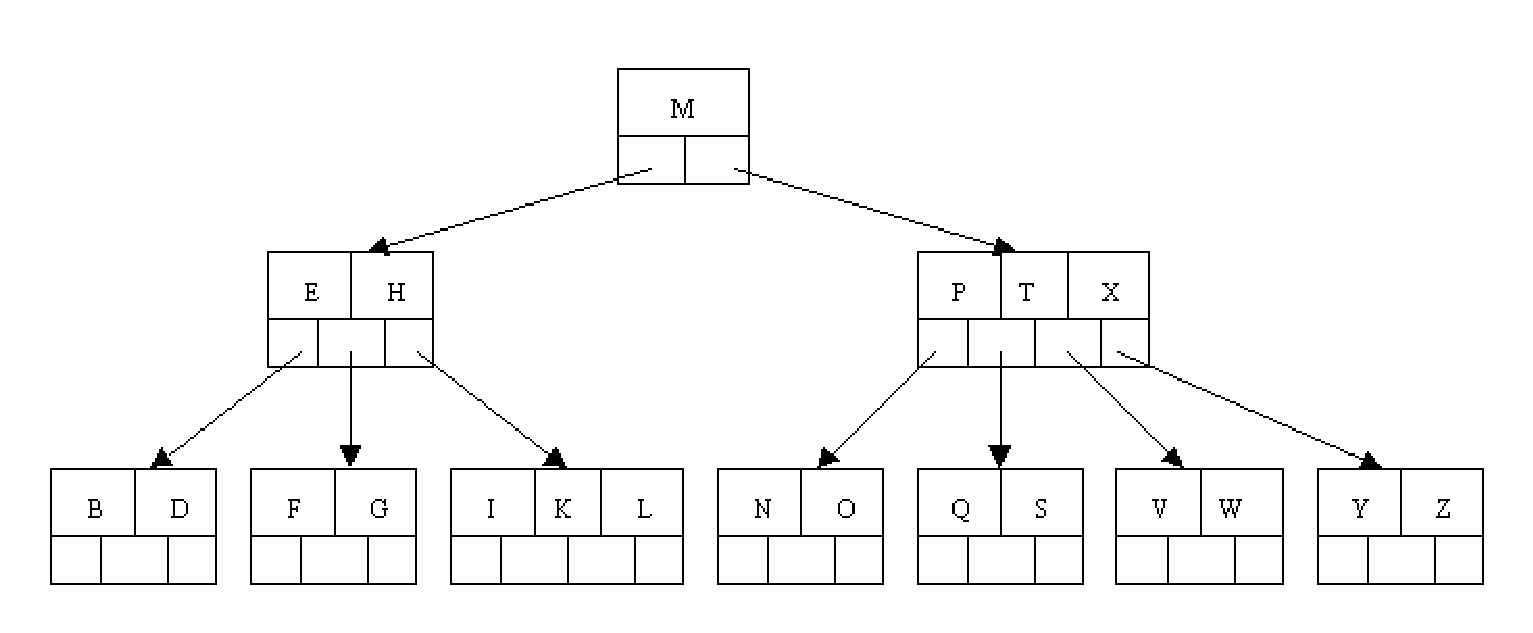
\includegraphics[scale=0.5]{images/b-tree}
  \caption{A B-tree with letters, of order 2 or 3}
  \label{fig:Btree}
\end{figure}

\subsection{Algorithm for B-trees}
Given an order relation, it's easy to search the predecessor / successor,
but we can't guarantee that any of them is the nearest.
Then we need to keep looking, to ensure we have the nearest point.
Since we're using a relation of lexicographical order,
we can stop looking for points, 
when the difference between the first coordinate
is greater than the minimum distance found.

\begin{algorithm}[t]
  \KwData{T: B-tree with the points, p: point to find its nearest neighbor}
  \KwResult{the nearest neighbor of p}
  x = find-node-of(p)\;
  \lIf{x exist}{return p\;}
  ans = $\emptyset$\;
  r = s = p\;
  \While{r != $\emptyset$ or s != $\emptyset$}{
    r = predecessor of r on T\;
    \lIf{r is colser to p than ans}{ans = r\;}
    x = find-node-of(r)\;
    \uIf{x is a leaf}{
      \ForEach{r child of x}{\lIf{r is colset to p than ans}{ans = r}}
      r = first-child of x\;
    }
    \lIf{distance in x from r to p is greater than distance between ans and p}{r = $\emptyset$}
    s = successor of s on T\;
    \lIf{s is colser to p than ans}{ans = s\;}
    x = find-node-of(s)\;
    \uIf{x is a leaf}{
      \ForEach{s child of x}{\lIf{s is closer to p than ans}{nas = r}}
      s = x.last-child\;
    }
    \lIf{distance in x from s to p is greater than distance between ans and p}{s = $\emptyset$}    
  }
  \caption{Nearest Neighbor in B-tree}
\end{algorithm}

\section{Quadtree}
A quadtree is a tree data structure in which each internal node has exactly four children. 
Quadtrees are most often used to partition a two-dimensional space by recursively 
subdividing it into four quadrants or regions. 
The regions may be square or rectangular, or may have arbitrary shapes. 
\begin{enumerate}
\item They decompose space into adaptable cells
\item Each cell (or bucket) has a maximum capacity. When maximum capacity is reached, the bucket splits
\item The tree directory follows the spatial decomposition of the quadtree.
\end{enumerate}
It can be seen in Figure~\ref{fig:quadtree},
the partition plane being performed by a quadtree with capacity 1

\begin{figure}[h!]
  \centering
  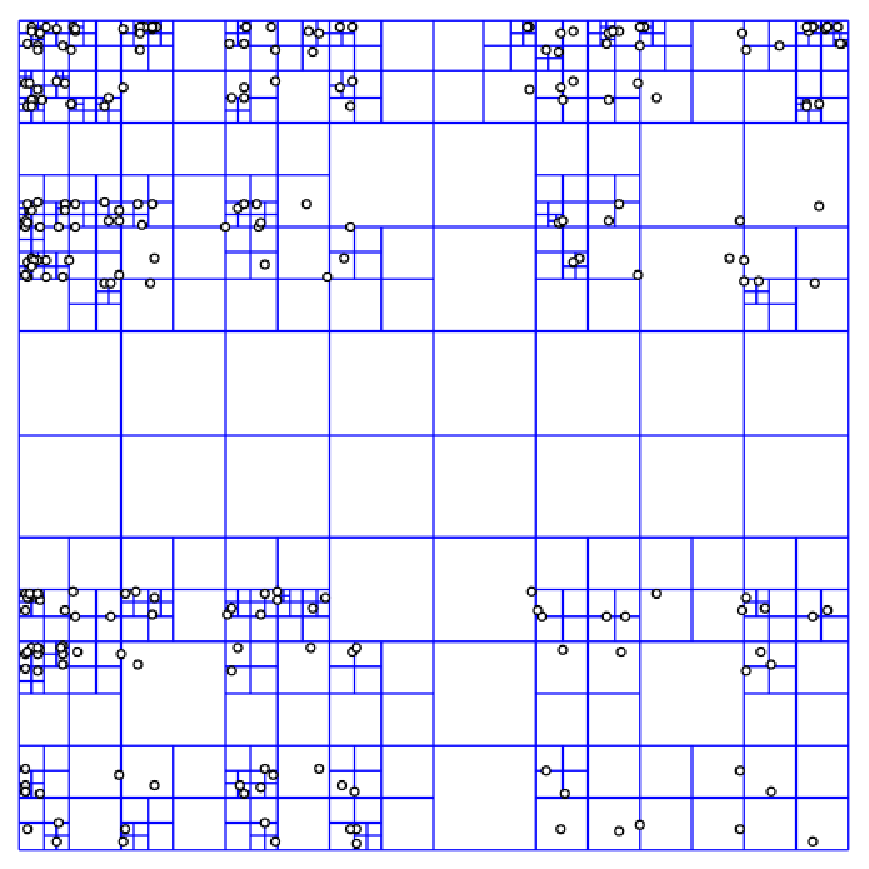
\includegraphics[scale=0.5]{images/point-quadtree}
  \caption{A point quadtree with point data. Bucket capacity 1}
  \label{fig:quadtree}
\end{figure}
To structure the points, we use quadtree with overlap,
this is that each quadrant contains a part of has rightful

\subsection{Algorithm for Quadtrees}
To find the nearest neighbor in a quadtree,
we need to compare the given point with the center of the quadtree,
and determine the next quadrant according to their position.
Until the quadrant in which we are, no contains more children.
To ensure that the point found is the nearest,
this would have to be closer to either side of the quadrant.

\section{Experimental Results}
Experiments were performed in a computer with Debian 8 'Jessie'
and characteristics specified in Table~\ref{tab:cpu}.

\begin{table}[h]
  \caption{CPU characteristics}
  \label{tab:cpu}
  \begin{center}
    \begin{tabular}{|l|r|}
      \hline
      Architecture:        & i686 \\
      CPU op-mode(s):      & 32-bit, 64-bit \\
      Byte Order:          & Little Endian \\
      CPU(s):              & 2 \\
      Thread(s) per core:  & 1 \\
      Core(s) per socket:  & 2 \\
      Socket(s):           & 1 \\
      Vendor ID:           & GenuineIntel \\
      CPU family:          & 6 \\
      Model:               & 15 \\
      Stepping:            & 13 \\
      CPU MHz:             & 1861.822 \\
      \hline
    \end{tabular}
  \end{center}
\end{table}
All the soucre code used for this test is available on
\url{https://github.com/ma1t05/EdDCpp_Proyect}.

The following experiments were performed
a set of \textit{k} points distributed uniformly in the plane was created,
for $k = 100,200,\ldots,1000$, to measure the setup time, and the memory uset to storage the structure, the results can be seen in Figures~\ref{fig:setup} and \ref{fig:memory}.
\begin{figure}[h!]
  \caption{Time Setup}
  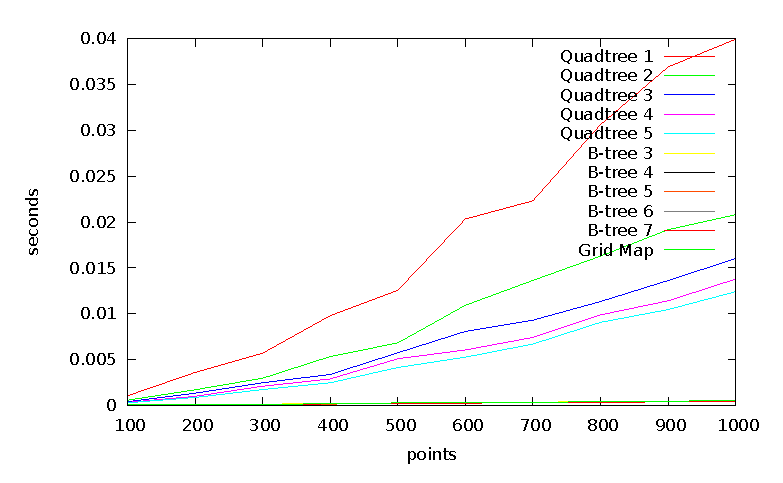
\includegraphics[scale=1.25]{images/setup}
  \label{fig:setup}
  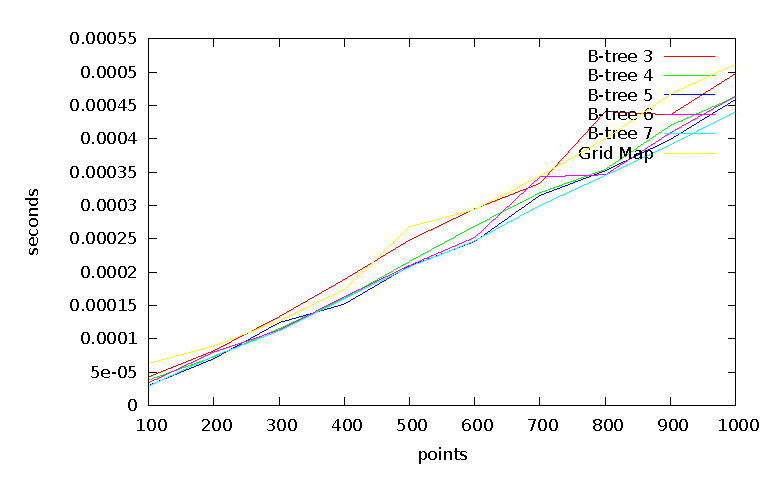
\includegraphics[scale=1.25]{images/setup_comparison}
\end{figure}[h!]
\begin{figure}
  \caption{Memory Usage}
  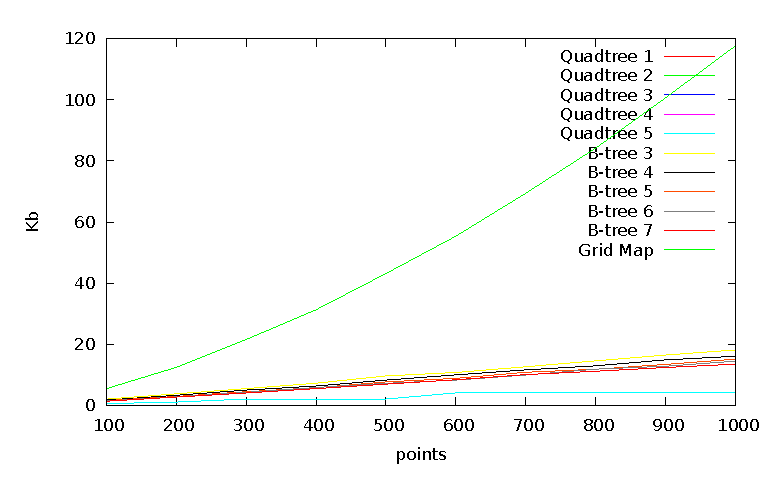
\includegraphics[scale=1.25]{images/memory}
  \label{fig:memory}
  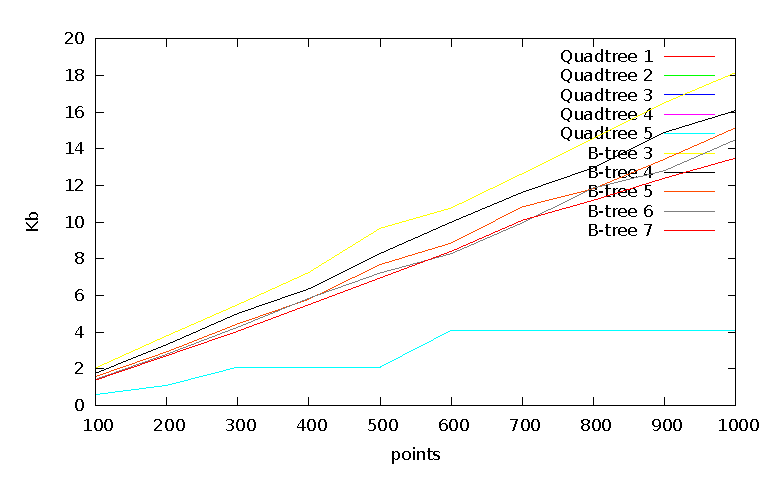
\includegraphics[scale=1.25]{images/memory_comparison}
\end{figure}

For $k = 1000$, we did a search of \textit{l} points, with $l = 1000,2000,\ldots,10000$, to see how the time behaves.

\section{Conclusions}
We can clearly see that the most advisable structure is the B-tree,
because it has a search time similar to the grid map (which is the lowest),
but it requires less memory, which increases linearly, not quadratic.
And regarding the quadtree, the only disadvantage it takes is the use of memory, 
the memory for B-tree apparently grows linearly, 
while the memory of the quadtree apparently grows logarithmically in some cases.
Our conclusions are based on having uniformly distributed points,
for future work, we could try other distributions for the points.
% Acknowledgments here
\ACKNOWLEDGMENT{%
We would like to thank Elisa Schaeffer for her helpful comments.
}% Leave this (end of acknowledgment)


% Appendix here
% Options are (1) APPENDIX (with or without general title) or 
%             (2) APPENDICES (if it has more than one unrelated sections)
% Outcomment the appropriate case if necessary
%
% \begin{APPENDIX}{<Title of the Appendix>}
% \end{APPENDIX}
%
%   or 
%
% \begin{APPENDICES}
% \section{<Title of Section A>}
% \section{<Title of Section B>}
% etc
% \end{APPENDICES}


% References here (outcomment the appropriate case) 

% CASE 1: BiBTeX used to constantly update the references 
%   (while the paper is being written).
%\bibliographystyle{ijocv081} % outcomment this and next line in Case 1
%\bibliography{Reporte_EDCpp.bib} % if more than one, comma separated
\begin{thebibliography}{9}

\bibitem{arya1994optimal}
  Arya, Sunil and Mount, David M and Netanyahu, N and Silverman, Ruth and Wu, Angela Y,
  \emph{\LaTeX: An optimal algorithm for approximate nearest neighbor searching in fixed dimensions},
  Proc. 5th ACM-SIAM Sympos. Discrete Algorithms,
  pages 573--582,
  1994.

\bibitem{samet1984quadtree}
  Samet, Hanan,
  \emph{\LaTeX: The quadtree and related hierarchical data structures},
  ACM Computing Surveys (CSUR),
  volume 16, number 2, pages 187--260,
  1984.

\bibitem{jadbabaie2003coordination}
  Jadbabaie, Ali and Lin, Jie and others,
  \emph{\LaTeX: Coordination of groups of mobile autonomous agents using nearest neighbor rules},
  Automatic Control, IEEE Transactions on
  volume 48, number 6, pages 988--1001,
  2003

\bibitem{roussopoulos1995nearest}
  Roussopoulos, Nick and Kelley, Stephen and Vincent, Fr{\'e}d{\'e}ric,
  \emph{\LaTeX: Nearest neighbor queries},
  ACM sigmod record,
  volume 24, number 2, pages 71--79,
  1995.

\bibitem{sproull1991refinements}
  Sproull, Robert F,
  \emph{\LaTeX: Refinements to nearest-neighbor searching ink-dimensional trees},
  Addison Wesley, Massachusetts,
  Algorithmica, volume 6, number 1-6, pages 579--589, Springer,
  1994.

\end{thebibliography}

% CASE 2: BiBTeX used to generate mypaper.bbl (to be further fine tuned)
%%%%%%%%%%%%%%%%%%%%%%%%%%%%%%%%%%%%%%%%%%%%%%%%%%%%%%%%%%%%%%%%%%%%%%%%%%%%%
%% Author template for INFORMS Journal on Computing (ijoc)
%% Mirko Janc, Ph.D., INFORMS, mirko.janc@informs.org
%% ver. 0.95, December 2010
%%%%%%%%%%%%%%%%%%%%%%%%%%%%%%%%%%%%%%%%%%%%%%%%%%%%%%%%%%%%%%%%%%%%%%%%%%%%
%\documentclass[ijoc,blindrev]{informs3}
\documentclass[ijoc,nonblindrev]{informs3} % current default for manuscript submission

%%\OneAndAHalfSpacedXI
\OneAndAHalfSpacedXII % current default line spacing
%%\DoubleSpacedXII
%%\DoubleSpacedXI

% If hyperref is used, dvi-to-ps driver of choice must be declared as
%   an additional option to the \documentclass. For example
%\documentclass[dvips,ijoc]{informs3}      % if dvips is used
%\documentclass[dvipsone,ijoc]{informs3}   % if dvipsone is used, etc.

% Private macros here (check that there is no clash with the style)

% Natbib setup for author-year style
\usepackage{natbib}
 \bibpunct[, ]{(}{)}{,}{a}{}{,}%
 \def\bibfont{\small}%
 \def\bibsep{\smallskipamount}%
 \def\bibhang{24pt}%
 \def\newblock{\ }%
 \def\BIBand{and}%

%% Setup of theorem styles. Outcomment only one. 
%% Preferred default is the first option.
\TheoremsNumberedThrough     % Preferred (Theorem 1, Lemma 1, Theorem 2)
%\TheoremsNumberedByChapter  % (Theorem 1.1, Lema 1.1, Theorem 1.2)

%% Setup of the equation numbering system. Outcomment only one.
%% Preferred default is the first option.
\EquationsNumberedThrough    % Default: (1), (2), ...
%\EquationsNumberedBySection % (1.1), (1.2), ...

% In the reviewing and copyediting stage enter the manuscript number.
\MANUSCRIPTNO{42} % When the article is logged in and DOI assigned to it,
                 %   this manuscript number is no longer necessary

%%%%%%%%%%%%%%%%
\begin{document}
%%%%%%%%%%%%%%%%

% Outcomment only when entries are known. Otherwise leave as is and 
%   default values will be used.
%\setcounter{page}{1}
%\VOLUME{00}%
%\NO{0}%
%\MONTH{Xxxxx}% (month or a similar seasonal id)
\YEAR{2015}% e.g., 2005
%\FIRSTPAGE{000}%
%\LASTPAGE{000}%
%\SHORTYEAR{00}% shortened year (two-digit)
%\ISSUE{0000} %
%\LONGFIRSTPAGE{0001} %
%\DOI{10.1287/xxxx.0000.0000}%

% Author's names for the running heads
% Sample depending on the number of authors;
% \RUNAUTHOR{Jones}
% \RUNAUTHOR{Jones and Wilson}
% \RUNAUTHOR{Jones, Miller, and Wilson}
% \RUNAUTHOR{Jones et al.} % for four or more authors
% Enter authors following the given pattern:
\RUNAUTHOR{Maltos}

% Title or shortened title suitable for running heads. Sample:
% \RUNTITLE{Bundling Information Goods of Decreasing Value}
% Enter the (shortened) title:
\RUNTITLE{Structs \& Algs for NNS in 2D}

% Full title. Sample:
% \TITLE{Bundling Information Goods of Decreasing Value}
% Enter the full title:
\TITLE{Structures and Algorithms for Nearest Neighbor Search in two dimensions}

% Block of authors and their affiliations starts here:
% NOTE: Authors with same affiliation, if the order of authors allows, 
%   should be entered in ONE field, separated by a comma. 
%   \EMAIL field can be repeated if more than one author
\ARTICLEAUTHORS{%
\AUTHOR{Luis Maltos}
\AFF{Programa de Posgrado en Ingenier\'ia de Sistemas, UANL \EMAIL{luis.maltosor@uanl.edu.mx}, \URL{}}
% Enter all authors
} % end of the block

\ABSTRACT{%
  Consider a set \textit{S} of \textit{n} data points in real 2-dimensional space, 
  where distances are measured using Euclidean metric.
  In nearest neighbor searching, we preprocess S into a data structure,
  so that given any query point \textit{q} $\in R^2$,
  is the closest point of \textit{S} to \textit{q} can be reported quickly.
  

}%

% Sample 
%\KEYWORDS{deterministic inventory theory; infinite linear programming duality; 
%  existence of optimal policies; semi-Markov decision process; cyclic schedule}

% Fill in data. If unknown, outcomment the field
\KEYWORDS{nearest neighbor searching}
%\HISTORY{}

\maketitle
%%%%%%%%%%%%%%%%%%%%%%%%%%%%%%%%%%%%%%%%%%%%%%%%%%%%%%%%%%%%%%%%%%%%%%

% Samples of sectioning (and labeling) in IJOC
% NOTE: (1) \section and \subsection do NOT end with a period
%       (2) \subsubsection and lower need end punctuation
%       (3) capitalization is as shown (title style).
%
%\section{Introduction.}\label{intro} %%1.
%\subsection{Duality and the Classical EOQ Problem.}\label{class-EOQ} %% 1.1.
%\subsection{Outline.}\label{outline1} %% 1.2.
%\subsubsection{Cyclic Schedules for the General Deterministic SMDP.}
%  \label{cyclic-schedules} %% 1.2.1
%\section{Problem Description.}\label{problemdescription} %% 2.

% Text of your paper here
\section{Introduction.}
Nearest neighbor searching is the following problem: 
We are given a set S of n data points in a metric space, X,
and the task is to preprocess these points so that,
given any query point $q \in X$,
the data point nearest to \textit{q} can be reported quickly.
This is also called the closest-point problem and the post office problem.
Nearest neighbor searching is an important problem in a variety of applications, including 
statistics [Devroye and Wagner 1982],
pattern recognition and classification [Cover and Hart 1967; Duda and Hart 1973],
document retrieval [Deerwester et al. 1990],
data compression [Gersho and Gray 1991],
machine learning [Cost and Salzberg 1993],
multimedia databases [Flickner et al. 1995],
and knowledge discovery and data mining [Fayyad et al. 1996].

Hierarchical data structures are useful because of their ability to focus on the
interesting subsets of the data. 
This focusing results in an efficient representation and improved execution times and is thus
particularly useful for performing set operations

\section{Nearest Neighbor Searching using B-trees}

\subsection{Algorithm for B-trees}

\section{Quadtree}
The term quadtree is used to describe a class of hierarchical data structures whose
common property is that they are based on the principle of recursive decomposition of space.
They can be differentiated on the following bases: 
(1) the type of data that they are used to represent, 
(2) the principle guiding the decomposition process, and 
(3) the resolution (variable or not)


A quadtree is a tree data structure in which each internal node has exactly four children. 
Quadtrees are most often used to partition a two-dimensional space by recursively 
subdividing it into four quadrants or regions. 
The regions may be square or rectangular, or may have arbitrary shapes. 
This data structure was named a quadtree by Raphael Finkel and J.L. Bentley in 1974. 

In this section, we introduce the \textit{balanced box-decomposition tree} or BBD-tree,
which is a data structure used in our algorithm. 
It is among the general class of geometric data structures based on a hierarchical decomposition of space
into \textit{d}-dimensional rectangles whose sides are orthogonal to the coordinate axes.
The main feature of the BBD-tree is that it combines in one data structure two
important features that are present in these data structures.
This data structure recursively subdivides space by a hyperplane that is orthogonal to one
of the coordinate axes and that partitions the data points as evenly as possible.
As a consequence, as one descends any path in the tree, the cardinality of points
associated with the nodes on this path decreases exponentially.

\section{Grid}

Lorem ipsum dolor sit amet, consectetur adipisicing elit, sed do eiusmod
tempor incididunt ut labore et dolore magna aliqua. Ut enim ad minim
veniam, quis nostrud exercitation ullamco laboris nisi ut aliquip ex ea
commodo consequat. Duis aute irure dolor in reprehenderit in voluptate
velit esse cillum dolore eu fugiat nulla pariatur. Excepteur sint
occaecat cupidatat non proident, sunt in culpa qui officia deserunt
mollit anim id est laborum.

Sed ut perspiciatis unde omnis iste natus error sit voluptatem
accusantium doloremque laudantium, totam rem aperiam, eaque ipsa quae ab
illo inventore veritatis et quasi architecto beatae vitae dicta sunt
explicabo. Nemo enim ipsam voluptatem quia voluptas sit aspernatur aut
odit aut fugit, sed quia consequuntur magni dolores eos qui ratione
voluptatem sequi nesciunt. Neque porro quisquam est, qui dolorem ipsum
quia dolor sit amet, consectetur, adipisci velit, sed quia non numquam
eius modi tempora incidunt ut labore et dolore magnam aliquam quaerat
voluptatem. Ut enim ad minima veniam, quis nostrum exercitationem ullam
corporis suscipit laboriosam, nisi ut aliquid ex ea commodi consequatur?
Quis autem vel eum iure reprehenderit qui in ea voluptate velit esse
quam nihil molestiae consequatur, vel illum qui dolorem eum fugiat quo
voluptas nulla pariatur?

At vero eos et accusamus et iusto odio dignissimos ducimus qui
blanditiis praesentium voluptatum deleniti atque corrupti quos dolores
et quas molestias excepturi sint occaecati cupiditate non provident,
similique sunt in culpa qui officia deserunt mollitia animi, id est
laborum et dolorum fuga. Et harum quidem rerum facilis est et expedita
distinctio. Nam libero tempore, cum soluta nobis est eligendi optio
cumque nihil impedit quo minus id quod maxime placeat facere possimus,
omnis voluptas assumenda est, omnis dolor repellendus. Temporibus autem
quibusdam et aut officiis debitis aut rerum necessitatibus saepe eveniet
ut et voluptates repudiandae sint et molestiae non recusandae. Itaque
earum rerum hic tenetur a sapiente delectus, ut aut reiciendis
voluptatibus maiores alias consequatur aut perferendis doloribus
asperiores repellat.

\section{Experimental Results}

% Acknowledgments here
\ACKNOWLEDGMENT{%
We would like to thank Elisa Schaeffer for her helpful comments.
}% Leave this (end of acknowledgment)


% Appendix here
% Options are (1) APPENDIX (with or without general title) or 
%             (2) APPENDICES (if it has more than one unrelated sections)
% Outcomment the appropriate case if necessary
%
% \begin{APPENDIX}{<Title of the Appendix>}
% \end{APPENDIX}
%
%   or 
%
% \begin{APPENDICES}
% \section{<Title of Section A>}
% \section{<Title of Section B>}
% etc
% \end{APPENDICES}


% References here (outcomment the appropriate case) 

% CASE 1: BiBTeX used to constantly update the references 
%   (while the paper is being written).
%\bibliographystyle{ijocv081} % outcomment this and next line in Case 1
%\bibliography{<your bib file(s)>} % if more than one, comma separated

% CASE 2: BiBTeX used to generate mypaper.bbl (to be further fine tuned)
%\input{mypaper.bbl} % outcomment this line in Case 2

\end{document}


 % outcomment this line in Case 2

\end{document}


